\chapter{IMPLEMENTATION, INTEGRATION AND TEST PLAN}
% The \label{...}% enables to remove the small indentation that is generated, always leave the % symbol.
\label{ch:IV}%
In this section, we specify the order of implementation of each component with a Gantt diagram.
\section{Implementation and Component Integration}
\label{sec:componentIntegration}%
The sequence of component implementation illustrated in the Gantt diagram refers to a relative time and not to an absolute one. All the components can actually be implemented in parallel by using the interface already provided in this document. \\
In particular, the best idea would be to provide all the methods of the interfaces with a dummy implementation that can be immediately used. After the single component has been implemented it can easily be integrated with the other ones since it already has a defined interface.\\
If the workforce is not big enough to implement all the components in parallel, the order of implementation should follow the described order of the Gantt diagram, hence, following all the start-to-start cascading relationships. 
% Maybe add description of why we chose this priority order
\subsubsection{eMSP Gantt Diagram}
\begin{figure}[H]
    \begin{center}
    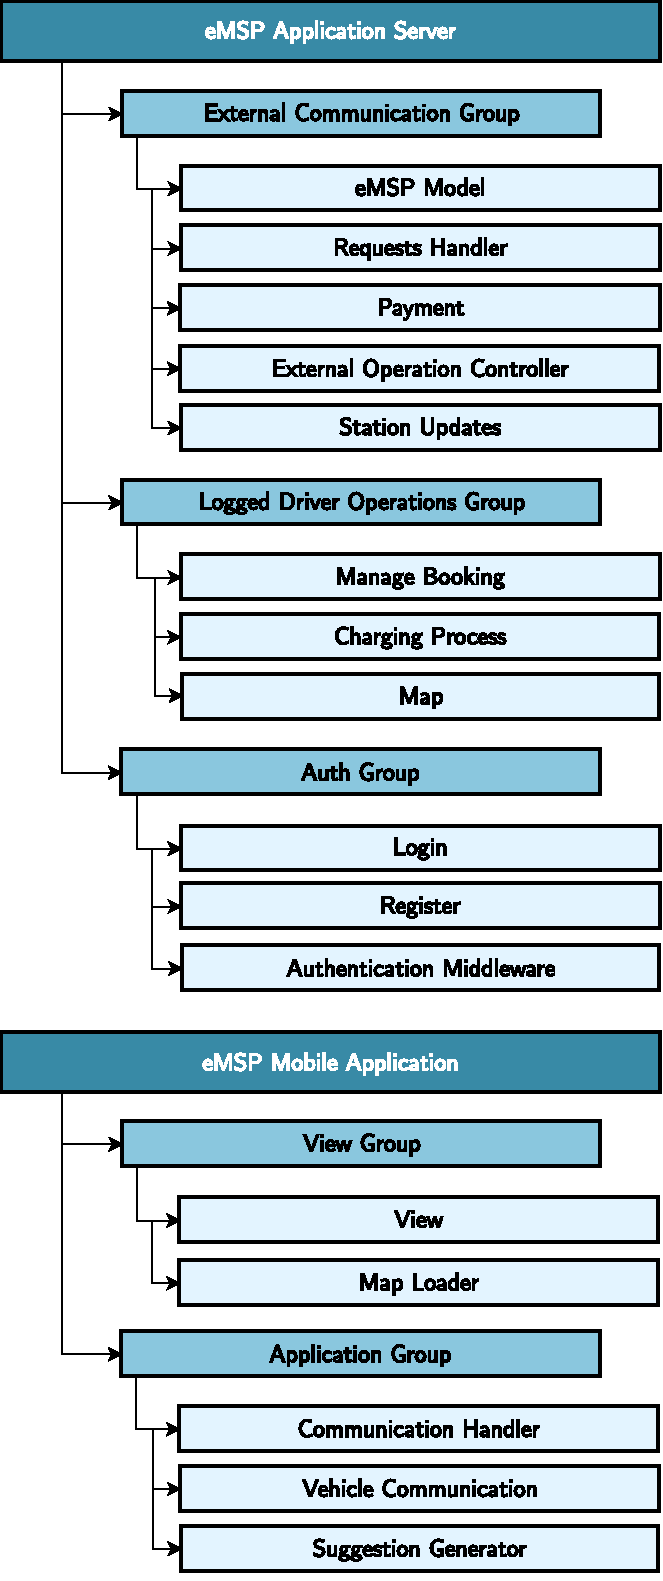
\includegraphics[
        width=\textwidth,
        height=0.75\textheight,
        keepaspectratio]{Gantt/eMSP Gantt}
    \caption{eMSP Gantt Diagram}
    \label{fig:eMSPGantt}
    \end{center}
\end{figure}

\subsubsection{CPMS Gantt Diagram}
\begin{figure}[H]
    \begin{center}
    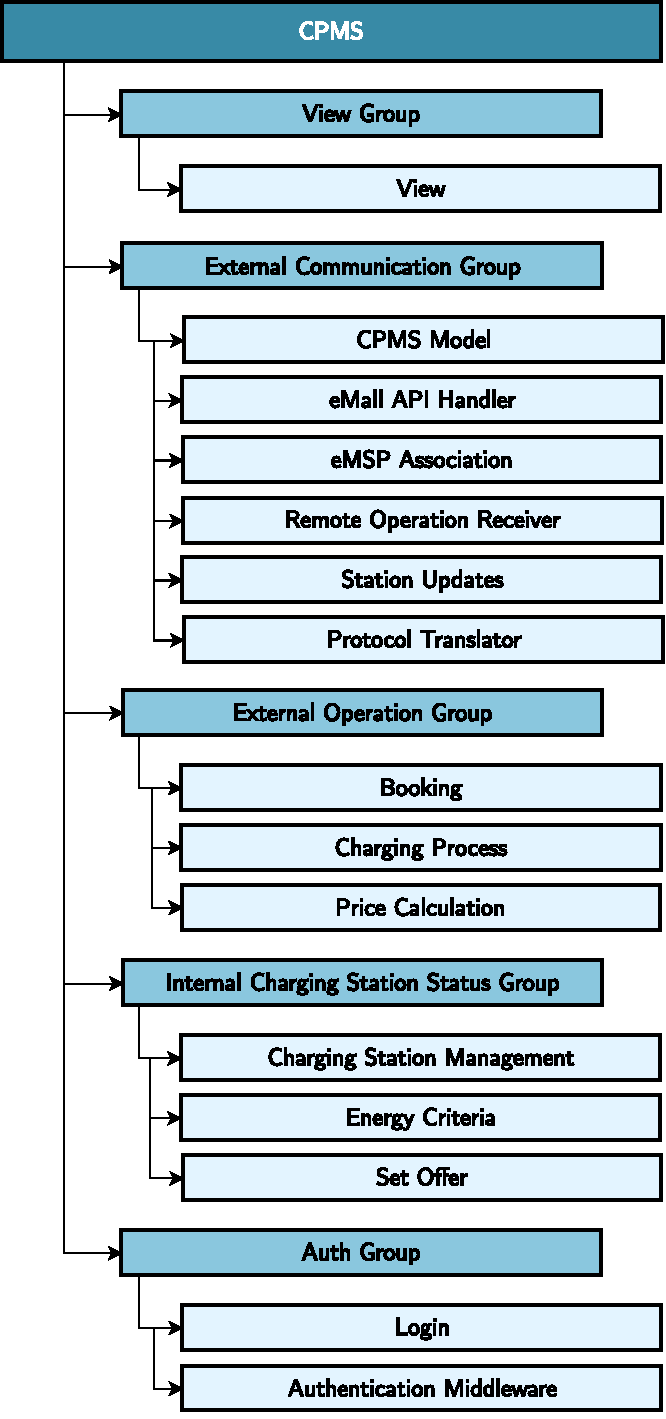
\includegraphics[
        width=\textwidth,
        height=0.75\textheight,
        keepaspectratio]{Gantt/CPMS Gantt}
    \caption{CPMS Gantt Diagram}
    \label{fig:CPMSGantt}
    \end{center}
\end{figure}
\newpage
\section{System Testing}
\label{sec:systemTesting}%
Since all the components could be developed in parallel, a good practice would be to use a TDD approach for the integration testing of the components. This involves writing a test for each interface method of each component as the interface is being developed. These tests will initially fail and only pass once the component has been implemented. In addition, unit testing should be performed for each component after implementation. This means that the testing phase will be integrated throughout the entire implementation process, rather than just at the end.
Overall we can split the testing phase into different parts:
\begin{enumerate}
    \item \textbf{Interfaces test writing: }Write tests for each interface method. All of them should fail.
    \item \textbf{Integration testing: }After a single component is developed and has replaced its stub, it should pass the test for its external interface.
    \item \textbf{Unit testing: }After a single component is developed, the developer should write tests in order to assure that every function inside that component is working in the proper way.
    \item \textbf{Performance testing: }After all the components have been developed and integrated, then there should be performance testing to make sure that there aren't any bottlenecks.
    \item \textbf{Load testing: }Load testing should be done in order to avoid bugs such as memory leaks or buffer overflows. There is also the possibility to test the system in order to understand how long it can resist at the maximum load.
    \item \textbf{Stress testing: }Stress testing is used to make sure that the system recovers carefully from a failure.
    \item \textbf{Networking testing: }Networking testing is used to make sure that the system can maintain its behaviour in case of a down node.
    \item \textbf{Acceptance testing: }This part should be the last part of the project, done with the stakeholders. It should check if the project respects the requirements and if the system satisfies the assignment.
\end{enumerate}